\documentclass[10pt, landscape, a4paper]{article}

\usepackage{fontspec}
\usepackage[english]{babel}
\babelfont{rm}{Noto Sans}
\babelfont{sf}{Noto Sans}

\usepackage{amsmath}
\usepackage{amssymb}
\usepackage{hyperref}
\usepackage{url}
\usepackage{graphicx}
\usepackage{geometry}
\usepackage{enumitem}
\usepackage{parskip}
\usepackage{chemfig}
\usepackage{pdfpages}
\usepackage{xcolor}
\usepackage{tikz}
\usepackage{fancybox}
\usepackage{makecell}
\usepackage{pgfplots}
\usepackage{ulem}
\usepackage{wrapfig}
\usepackage{subcaption}
\usepackage{esvect}
\usepackage{siunitx}
\usepackage{mathtools}
\usepackage{varwidth}
\usepackage{multicol}
\usepackage{titlesec}
\usepackage{bm}

\usetikzlibrary{arrows}
\usetikzlibrary{arrows.meta}
\usetikzlibrary{decorations.pathreplacing}
\pgfplotsset{compat=1.18}
\definecolor{darkgreen}{rgb}{0.0, 0.6, 0.0}

% ============= GEOMETRY =============
\geometry{
    a4paper,
    landscape,
    left=0.5cm,
    right=0.5cm,
    top=1.5cm, 
    bottom=0.5cm,
    footskip=0cm
}

\setlist{nosep, leftmargin=*} 

\AtBeginDocument{
  \setlength{\abovedisplayskip}{3pt}
  \setlength{\belowdisplayskip}{3pt}
  \setlength{\abovedisplayshortskip}{0pt}
  \setlength{\belowdisplayshortskip}{0pt}
}

% ============= HEADER & TITLES =============
\usepackage{fancyhdr}
\pagestyle{fancy}
\fancyhf{}
\rhead{\small Systems Modelling Cheat Sheet}
\lhead{\small Matteo Frongillo}
\cfoot{\small \thepage}
\renewcommand{\headrulewidth}{0pt}
\setlength{\headsep}{2pt}

% Aggressive spacing reduction for titles
\titlespacing*{\section}{0pt}{2pt}{1pt}
\titlespacing*{\subsection}{0pt}{2pt}{1pt}
\titlespacing*{\subsubsection}{0pt}{1pt}{1pt}

\titleformat{\section}{\normalfont\large\bfseries\color{black}}{}{0em}{}
\titleformat{\subsection}{\normalfont\normalsize\bfseries\color[HTML]{007AFF}}{}{0em}{}
\titleformat{\subsubsection}{\normalfont\small\bfseries\color[HTML]{007355}}{}{0em}{}

% ============= META DATA =============
\newcommand{\pdftitle}[1]{\hypersetup{
  colorlinks=true,
  linkcolor=black,
  urlcolor=blue,
  pdftitle={#1},
  pdfauthor={Matteo Frongillo}
}}

% ============= RENEW COMMANDS =============

\makeatletter
\renewcommand{\author}[1]{%
  \def\@author{%
    #1\\
    \parbox{\textwidth}{%
      \centering
      \small Last update: \today
    }
  }%
}
\makeatother

\let\emptyset\varnothing

\makeatletter
\pgfmathdeclarefunction{arctan}{1}{%
    \begingroup
    \pgfmathparse{rad(atan(#1))}%
    \endgroup
}
\makeatother

% ============= NEW COMMANDS =============

\newcommand{\figbox}[1]{ 
    \begin{figure*}[ht!]        
        \begin{center}            
            \fbox{\begin{varwidth}{\textwidth} #1 \end{varwidth}}        
        \end{center}    
    \end{figure*}
}

\newcommand{\wrapfill}{
    \par
    \ifnum \value{WF@wrappedlines} > 0
        \addtocounter{WF@wrappedlines}{-1}%
        \null\vspace{
            \arabic{WF@wrappedlines}
            \baselineskip
        }
        \WFclear
    \fi
    \phantom{}
}

\ExplSyntaxOn
\DeclareDocumentCommand{\integral}{d[] d[] d[] d[]}
{
    \IfNoValueTF{#3}{
        \IfNoValueTF{#4}{
            \displaystyle \int #1\,d#2
        }{
            \text{Error: either 2 or 4 arguments must be provided}
        }
    }{
        \IfNoValueTF{#4}{
            \text{Error: either 2 or 4 arguments must be provided}
        }{
            \displaystyle
            \int\limits
                \IfNoValueF{#1}{\c_math_subscript_token{#1}}
                ^{\IfNoValueTF{#2}{}{#2}}
                #3\, d#4
        }
    }
}
\ExplSyntaxOff

\newcommand*\circled[1]{\tikz[baseline=(char.base)]{
            \node[shape=circle,draw,inner sep=1pt] (char) {\small #1};}} % Reduced inner sep

\makeatletter
\newcommand*{\rom}[1]{\expandafter\@slowromancap\romannumeral #1@}
\makeatother

\newcommand{\difference}{\,\backslash\,}
\newcommand{\rem}{\underline{Remark}: }
\newcommand{\nots}{\underline{Notation}: }
\newcommand{\note}{\underline{Note}: }
\newcommand{\prf}{\underline{Proof}: }
\newcommand{\exs}{\underline{Example}: }
\newcommand{\defs}{\underline{Definition}: }
\newcommand{\wrn}{\underline{Warning}: }
\newcommand{\sht}{\ |\ }
\newcommand{\pph}[1]{\paragraph{#1} \phantom{}\\}
\newcommand{\dm}{\displaystyle}
\newcommand{\rad}{^{\mathrm{c}}}
\newcommand{\dsum}[2]{\displaystyle \sum_{#1}^{#2}}
\newcommand{\dx}[2]{\dfrac{{\mathrm{d}}^{#1}{#2}}{\mathrm{d}x^{#1}}}

% ============= DOCUMENT CONTENT =============

\title{Systems Modelling}
\author{Matteo Frongillo}
\date{\today}

\begin{document}

\setlength{\columnsep}{0.5cm}

\begin{multicols*}{3}

\section{SW 1: Introduction}
\subsection{Model's three properties}
\begin{itemize}
    \item \textbf{Mapping}: models act as a representation of natural or artificial originals and can be models in turn;
    \item \textbf{Reduction}: models function as abstraction. They do not capture every attribute of the original; instead, they isolate and retain only those attributes relevant to the specific objective, intentionally omitting detail to manage complexity and focus on the problem at hand;
    \item \textbf{Pragmatic}: models function as utilitarian substitutes. They do not replace the original universally but serve as a representative for a specific user (subject), within a defined time frame, and for a particular purpose or operation.   
\end{itemize}

\textbf{Example}
\begin{center}
    \includegraphics[width=.6\linewidth]{media/sw1_inclinedplane.png}
\end{center}
\begin{itemize}
    \item \textbf{Generaliz.}: point mass sliding down an inclined plane;
    \item \textbf{Mapping}: box as mass, conveyor slope as an angle $\theta$, vertical drop as height $h$, gravity;
    \item \textbf{Reduction}: no structure flexibility, no air movement, no friction, no rollers\ $\rightarrow$\ flat plane;
    \item \textbf{Pragmatic}: it allows $a,v_f,t$ of the box to be calculated, it enables the prediction of how to build a belt mockup.  
\end{itemize}

\subsection{Digital representation}
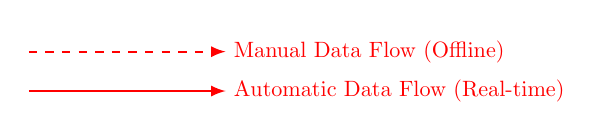
\begin{tikzpicture}
    \draw[-latex, dashed, thick, red] (0,0) -- (2.5,0) node[right, scale=0.8] {Manual Data Flow (Offline)};
    \draw[-latex, thick, red] (0,-.5) -- (2.5,-.5) node[right, scale=0.8] {Automatic Data Flow (Real-time)};
\end{tikzpicture}
\subsubsection{Digital model (simulation)}
No direct connection between digital and physical object:
\begin{center}
    \includegraphics[width=.6\linewidth]{media/sw1_digitalmodel.png}
\end{center}

\subsubsection{Digital shadow}
Unidirectional, automated data flow from physical object to digital model:
\vspace*{-.3cm}
\begin{center}
    \includegraphics[width=.9\linewidth]{media/sw1_digitalshadow.png}
\end{center}

\subsubsection{Digital twin}
Automated data exchange between physical object and model:
\begin{center}
    \includegraphics[width=.7\linewidth]{media/sw1_digitaltwin.png}
\end{center}

\subsection{Role of time}
\subsubsection{Stationary behavior}
Steady-state operation: $\dot{m}_\alpha = \dot{m}_\omega$

\subsubsection{Dynamic behavior}
Non stationary/transient/unsteady: $\dfrac{dm}{dt} = \dot{m}_\alpha - \dot{m}_\omega$

\subsection{Governing dynamics}
\subsubsection{Empirical (black box)}
\noindent
\begin{minipage}[c]{0.65\linewidth}
    Data based, without direct physics link.
    (ex: machine learning, fitting of functions)
\end{minipage}
\hfill
\begin{minipage}[c]{0.3\linewidth}
    \centering
    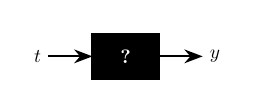
\begin{tikzpicture}[scale=0.7, every node/.style={scale=0.7}]
        \draw[thick, -{Stealth}] (-0.8, 0.4) -- (0, 0.4) node[pos=0, left] {$t$};
        \draw[thick, -{Stealth}] (1.2, 0.4) -- (2.0, 0.4) node[pos=1, right] {$y$};
        \draw[thick, fill=black] (0,0) rectangle (1.2,0.8);
        \node[white] at (0.6,0.4) {\textbf{?}};
    \end{tikzpicture}
\end{minipage}

\subsubsection{Physics-based (white box)}
\noindent
\begin{minipage}[c]{0.65\linewidth}
    Based on physical laws.\\
    (ex: conservation of mass)
\end{minipage}
\hfill
\begin{minipage}[c]{0.3\linewidth}
    \centering
    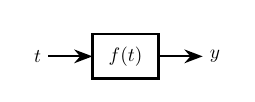
\begin{tikzpicture}[scale=0.7, every node/.style={scale=0.7}]
        \draw[thick, -{Stealth}] (-0.8, 0.4) -- (0, 0.4) node[pos=0, left] {$t$};
        \draw[thick, -{Stealth}] (1.2, 0.4) -- (2.0, 0.4) node[pos=1, right] {$y$};
        \draw[thick] (0,0) rectangle (1.2,0.8);
        \node at (0.6,0.4) {$f(t)$};
    \end{tikzpicture}
\end{minipage}

\subsubsection{Grey-box (hybrid)}
\noindent
\begin{minipage}[c]{0.65\linewidth}
    Combining physics and data\\ parameters.
\end{minipage}
\hfill
\begin{minipage}[c]{0.3\linewidth}
    \centering
    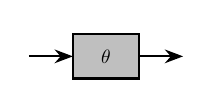
\begin{tikzpicture}[scale=0.7, every node/.style={scale=0.7}]
        \draw[thick, -{Stealth}] (-0.8, 0.4) -- (0, 0.4);
        \draw[thick, -{Stealth}] (1.2, 0.4) -- (2.0, 0.4);
        \draw[thick, fill=gray!50] (0,0) rectangle (1.2,0.8);
        \node at (0.6,0.4) {$\theta$};
    \end{tikzpicture}
\end{minipage}

\subsection{Role of space}
\subsubsection{Point model (0D)}
Assumes the whole system is perfectly mixed.
(ex: ideal mixer with isotropic distribution).
Software: Excel, MATLAB

\newcolumn
\subsubsection{Linked point}
Connects several simple models together to create a basic network or layout.
(ex: space shown via linking of 0D-models).
Software: Simulink, Modelica

\subsubsection{Spatial model (1-3D)}
Considers real position of state variables or entities;
spatial relationships affect the dynamics.
(ex: real mixer with anisotropic, heterogeneous distribution).
Software: COMSOL, ANSYS, AutoCAD, REVIT\\
\textbf{Example with a heat pump}
\begin{itemize}
    \item \textbf{Purpose}: digital shadow $\to$\ automated data;
    \item \textbf{Governing dynamics}: physics-based $\to$\ based on thermodyn. laws;
    \item \textbf{Time}: time dependent, dynamic behavior $\to$\ heating load, power of the hp, on/off cycles;
    \item \textbf{Space}: linked point $\to$\ el. inputs, thermal\\energy exchange, 4 components to monitor.
\end{itemize}

\subsection{Solvability of models}
\subsubsection{Analytical}
Closed formula as solution. Only for simple problems.
\[A=\dfrac{x^3}{3}\Big|_0^2 = \dfrac{8}{3}\]

\subsubsection{Numerical}
Numerical approximation. For complex problems.
\[A\approx \dsum{i=1}{n} f(x_i) dx \approx 2.6667 \]

\subsection{Further modelling properties}
\subsubsection{Linear vs Non-linear}

\noindent
\begin{minipage}[t]{0.48\linewidth}
    \centering
    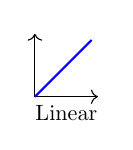
\begin{tikzpicture}[scale=0.4]
        \draw[->] (0,0) -- (2,0);
        \draw[->] (0,0) -- (0,2);
        \draw[blue, thick] (0,0) -- (1.8,1.8);
        \node[scale=.8] at (1,-0.5) {Linear};
    \end{tikzpicture}
\end{minipage}
\hfill
\begin{minipage}[t]{0.48\linewidth}
    \centering
    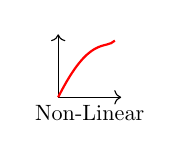
\begin{tikzpicture}[scale=0.4]
        \draw[->] (0,0) -- (2,0);
        \draw[->] (0,0) -- (0,2);
        \draw[red, thick] (0,0) .. controls (1,2) and (1.5,1.5) .. (1.8,1.8);
        \node[scale=.8] at (1,-0.5) {Non-Linear};
    \end{tikzpicture}
\end{minipage}

\subsubsection{Continuity vs Differentiability}
\noindent
\begin{minipage}[t]{0.31\linewidth}
    \centering
    \scalebox{0.7}{
    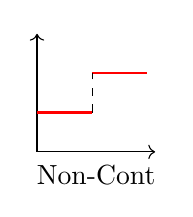
\begin{tikzpicture}
        \draw[->] (0,0) -- (1.5,0); \draw[->] (0,0) -- (0,1.5);
        \draw[red, thick] (0,0.5) -- (0.7,0.5);
        \draw[red, thick] (0.7,1.0) -- (1.4,1.0);
        \draw[dashed] (0.7,0.5) -- (0.7,1.0);
        \node at (0.75,-0.3) {Non-Cont};
    \end{tikzpicture}}
\end{minipage}
\hfill
\begin{minipage}[t]{0.31\linewidth}
    \centering
    \scalebox{0.7}{
    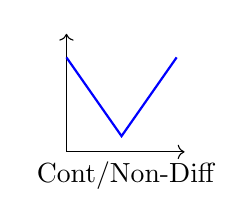
\begin{tikzpicture}
        \draw[->] (0,0) -- (1.5,0); \draw[->] (0,0) -- (0,1.5);
        \draw[blue, thick] (0,1.2) -- (0.7,0.2) -- (1.4,1.2);
        \node at (0.75,-0.3) {Cont/Non-Diff};
    \end{tikzpicture}}
\end{minipage}
\hfill
\begin{minipage}[t]{0.31\linewidth}
    \centering
    \scalebox{0.7}{
    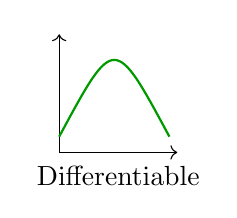
\begin{tikzpicture}
        \draw[->] (0,0) -- (1.5,0); \draw[->] (0,0) -- (0,1.5);
        \draw[darkgreen, thick] (0,0.2) .. controls (0.7,1.5) .. (1.4,0.2);
        \node at (0.75,-0.3) {Differentiable};
    \end{tikzpicture}}
\end{minipage}

\subsubsection{Deterministic vs Stochastic}
\noindent
\begin{minipage}[t]{0.48\linewidth}
    \centering
    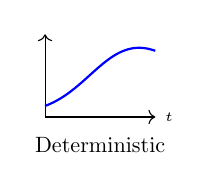
\begin{tikzpicture}[scale=0.7]
        \draw[->] (0,0) -- (2,0) node[right] {\tiny $t$};
        \draw[->] (0,0) -- (0,1.5);
        \draw[blue, thick] (0,0.2) to[out=20, in=160] (2,1.2);
        \node[scale=.8] at (1,-0.5) {Deterministic};
    \end{tikzpicture}
\end{minipage}
\hfill
\begin{minipage}[t]{0.48\linewidth}
    \centering
    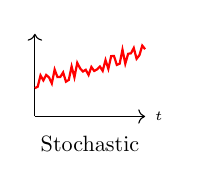
\begin{tikzpicture}[scale=0.7]
        \draw[->] (0,0) -- (2,0) node[right] {\tiny $t$};
        \draw[->] (0,0) -- (0,1.5);
        \draw[red, thick] plot[domain=0:2, samples=40] (\x, {0.6 + 0.3*\x + 0.15*rand});
        \node[scale=.8] at (1,-0.5) {Stochastic};
    \end{tikzpicture}
\end{minipage}

\subsection{Modelling approaches}
\subsubsection{Top-down}
Largest components broken down into smaller.
ex: marble block sculpture, railway network.\\
\circled{+} Efficient model, \circled{--} Misses details

\subsubsection{Bottom-up}
Individual components combined into larger.
ex: LEGO model, human body.\\
\circled{+} Detailed model, \circled{--} Complex

\section{SW2: How to model a system}
\begin{enumerate}
    \item Problem formulation
    \item Mathematical representation
    \item Mathematical analysis
    \item Interpretation and evaluation of results
\end{enumerate}

\subsection{Problem formulation}
\subsubsection{Task 1 - Defining goals}
What do we want to achieve?\\
How well/closely does our model need to represent reality?\\
What could be the goals for this specific system?

\subsubsection{Task 2 - Characterize the system}
What are the relevant parameters and variables of the system?\\
What are the system boundaries?\\
What are the inputs and outputs of the system?

\subsubsection{Task 3 - Simplify and idealize the system}
Still reproduce the significant behaviors of the system, while reducing complexity.\\
Reduce model to the main parameters and variables (ex. for hp:
COP? Max. power? Avg power? Yearly values? Temperature levels?).

\subsection{Mathematical formulation}
\subsubsection{Task 1 - Identify fundamental theories and laws}
If no laws are available, use ad-hoc or empirical data to derive relationships:\\
Thermodynamic laws, material properties, ad-hoc\\
$P_{out} = COP(T_{amb})\cdot P_{in}$

\subsubsection{Task 2 - Derivation of relationships}
Transfer system into a mathematical formulation.\\
\textbf{Top-down (black/grey box)}:
Use generic relationship, data from measurement to determine parameters.
For more complex systems, add more parameters.
Use techniques such as machine learning.

\newcolumn
\textbf{Bottom-up}:
Detailed physical modelling of the device.
Physical laws to describe each component.
Exact geometry, material properties, boundary conditions.

\subsubsection{Task 3 - Reduce to standard mathematical problem}
Simple algebra, linear programming, differential equation, diffusion problem,
wave propagation, FEM problem, using suitable methods and software/programming tools.

\subsection{Interpretation and evaluation of the results}
\subsubsection{Task 1 - Calibration of results}
Use existing data to calibrate the model.

\subsubsection{Task 2 - Validation}
Check underlying physics law, such as energy or mass conservation,
compare to known solutions, look at extreme cases, compare to measured data.\\
$\to$\ What is it and why do we have to do it?

\textbf{Before the modelling}:\\
What do we model how?:
\vspace*{-0.2cm}
\begin{enumerate}[label=\alph*)]
    \item Aims: does the model describe the process under test?
    \item Output: does the model provide the required output to describe the process?
    \item Type: is the type of the model suitable to describe the process?
\end{enumerate}

\vspace*{-0.2cm}
\textbf{During modelling}:\\
Can we reproduce the measurements?\\
Does the model behave like to system under study?
\vspace*{-0.2cm}
\begin{enumerate}[label=\alph*), start=4]
    \item Fitting data: does the model reproduce the fitting data? How to measure accuracy?
    \item Reproducing novel data: does the model also predict novel measurement data correctly?
    \item Sensitivity analysis: does the model predict the behavior of the system correctly when system parameters are changed?
\end{enumerate}

\vspace*{-0.2cm}
\textbf{After modelling}:\\
Does the model also work with new data?
\vspace*{-0.2cm}
\begin{enumerate}[label=\alph*), start=7]
    \item System potentially changed.
    \item Differences in system behavior is only manifest in new experiments.
\end{enumerate}

\newcolumn
\section{SW 3: Data-based modelling}
\subsection{Linear regression}
Used to find a linear function $y=f(x)=a+bx$ that best fits a dataset ${(x_i,y_i)}$.
\subsubsection{Least squares method}
Minimize the sum of squared errors (SSE):
\[S=\sum_{i=1}(y_i - (a+bx_i))^2\]
If measurement uncertainties $\Delta y_i$ exist, weight the error:
\[S_i = \frac{y_i-y(x)}{\Delta y_i}\]

\subsubsection{Optimal parameter formulas}
Finding $a$ and $b$ when $S$ is minimal:
\[\frac{\partial S}{\partial a} = 0\quad ; \quad \frac{\partial S}{\partial b} = 0\]
Slope $b$:
\[b=\frac{\sum_i x_iy_i - \frac{1}{n}\left(\sum_i x_i\right)\left(\sum_i y_i\right)}{\sum_i x_i^2 - \frac{1}{n}\left(\sum_i x_i\right)^2}\]
Intercept $a$:
\[a=\bar{y} - b\bar{x}\]
where:
\[\bar{x} = \dfrac{\sum_i x_i}{n}\quad ; \quad \bar{y} = \dfrac{\sum_i y_i}{n}\]

\subsubsection{Quality of fit $\mathbf{\left(R^2\right)}$}
The coefficient of determination $R^2$ indicates the percentage of variation explained
by the model:
\[R^2 = \frac{\sum_i \left(y(x)-\bar{y}\right)^2}{\sum_i \left(y_i - \bar{y}\right)^2}\]
\vspace*{-0.2cm}
\begin{itemize}
    \item $R^2 = 1\ (100\%)$: the model explains all data;
    \item $R^2 = 0\ (0\%)$: the model doesn't (random).
\end{itemize}

\subsubsection{Multilinear regression}
Used when the target depends on multiple variables:
\[y(x_1,\dots,x_n) = a+b_1x_1 + \dots + b_nx_n = a + \sum_{j=1}^{n} b_j x_{j}\]

\subsection{Non-linear regression}
The goal is to fit data using non-linear functions when the underlying process is not linear.
\subsubsection{Linearization techniques}
\vspace{-.2cm}
\begin{center}
    \renewcommand{\arraystretch}{2}
    \begin{tabular}{|l|l|l|l|}
        \hline \small Function & Equation & Trasformation & Variables\\
        \hline \small Exp & $y=ae^{bx}$ & $\ln y = \ln a + bx$ & $x$ vs $\ln y$\\
        \hline \small Power & $y=ab^x$ & $\ln y = \ln a + x\ln b$ & $x$ vs $\ln y$\\[.5ex]
        \hline \small Inverse & $y=\dfrac{a}{x}$ & $\dfrac{1}{y} = \dfrac{x}{a}$ & $x$ vs $\dfrac{1}{y}$\\
        \hline \small \makecell[l]{Square\\offset} & $y=ax^2 + b$ & $y=a(x^2)+b$ & $x^2$ vs $y$\\
        \hline \small \makecell[l]{Root /\\Cubic} & $y=\sqrt{ax^3+b}$ & $y^2=ax^3+b$ & $x^3$ vs $y^2$\\
        \hline         
    \end{tabular}
\end{center}

\subsection{Maximum likelihood method (MLE)}
Determines the parameters of a probability distribution that best describes a dataset,
independent of histogram binning.
\subsubsection{Likelihood function}
Defines as the product of probability densities for all data points:
\[L(\sigma,\mu) = \prod_i f(x_i,\sigma,\mu)\]

\subsubsection{Log-likelihood}
To simplify calculation and avoid small numbers, minimize the negative logarithm:
\[-\log L = -\sum_i \log(f(x_i,\sigma,\mu))\]

\subsubsection{Common distribution}
\textbf{Normal distribution}:
\[f(x)=\dfrac{1}{\sigma\sqrt{2\pi}}\exp\left(-\dfrac{1}{2}\left(\dfrac{x-\mu}{\sigma}\right)^2\right)\]

\textbf{Weibull distribution (Reliability)}:
\[f(x) = \begin{cases}
    \lambda k (\lambda x)^{k-1} e^{-(\lambda x)^k}, &x>0\\
    0 &\text{else}
\end{cases}\]

\textbf{Weibull cumulative distribution function}
\[F(x) = \integral[-\infty][x][f(u)][u] = \begin{cases}
    1-e^{-(\lambda x)^k} & for x>0\\
    0 &\text{else}
\end{cases}\]
\newcolumn

\section{SW4: Modelling with ODEs}
\subsection{Fundamentals of ODEs}
An ODE contains functions of one independent variable and their derivatives.
\subsubsection{Ordinary (ODE)}
Involves one independent variable:
\[\dfrac{d^2x}{dt^2} = -g\]

\subsubsection{Partial (PDE)}
Involves multiple independent variables:
\[\dfrac{d^2u}{dt^2} = c^2\dfrac{d^2u}{dx^2}\]

\subsection{Analytical solution method}
\subsubsection{Separation of variables}
Used when terms involving $y$ and $x$ can be moved to opposite sides.

\subsubsection{Variation of parameters}
Used for inhomogeneous linear ODEs. General solution is the sum of the homogeneous
solution and a particular solution.

\subsection{Numerical solution methods}
\subsubsection{Euler method}
A simple iterative method to approximate ODEs defined as $\dfrac{df}{dx} = g(x)$.\\
The approximation uses the finite difference slope:
\[\dfrac{df}{dx} \approx \dfrac{f(x_0+\Delta x) - f(x_0)}{\Delta x}\]
Iterative steps:
\[f(x_0+\Delta x) = f(x_0)+g(x_0)\Delta x\]

\subsection{Modelling principles}
\subsubsection{Balance equations}
Based on the conservation principle:
\[\frac{d}{dt} f(t) = f(t_\alpha) - f(t_\omega)\]
\textbf{Example in a capacitor}
\[U_0 = U_R + U_C \Rightarrow U_0 = RI + \frac{Q}{C} = R\frac{dQ}{dt}+\frac{Q}{C}\]

\newcolumn
\subsubsection{Mechanics and forces}
Equation of motion is derived from Newton's second law $F_{net} = ma$.\\
\textbf{Example of a falling drop with drag}
\[m\dot{v}=mg-bv \Rightarrow v(t) = \frac{mg}{b}\left(1 - e^{-bt/m}\right)\]

\subsubsection{Growth and decay}
Describes processes where a quantity increases or decreases over time.
\[\frac{dN}{dt} = kN \Rightarrow N(t)=N_0e^{kt}\]
with half-time / doubling factor $\tau$:
\[\tau = \left|\frac{\ln 2}{k}\right|\]
\textbf{Example of logistic growth}
\[\frac{dN}{dt} = KN(t) - \frac{K}{K}N^2 \Rightarrow N(t) = \frac{L}{1+\left(\frac{L}{N_0}-1\right)e^{-kt}}\]

\subsubsection{Recipe to derive the equation of motion}
\begin{enumerate}
    \item Make a sketch of the situation;
    \item Define the coordinate system and select variables of interest;
    \item Identify all forces and momenta;
    \item Formulate the equation of motion;
    \item Solve it.
\end{enumerate}

\subsection{Linear algebra and systems of ODEs}
\subsubsection{Matrix representation}
System of equations:
\begin{gather*}
    a_{11}x_1 + a_{12}x_2+a_{13}x_3 = b_1\\
    a_{21}x_1 + a_{22}x_2+a_{23}x_3 = b_2\\
    a_{31}x_1 + a_{32}x_2+a_{33}x_3 = b_3
\end{gather*}
Matrix form ($Ax = b$):
\[
\begin{pmatrix}
    a_{11}&a_{12}&a_{13}\\
    a_{21}&a_{22}&a_{23}\\
    a_{31}&a_{32}&a_{33}
\end{pmatrix}
\begin{pmatrix}
    x_1\\
    x_2\\
    x_3
\end{pmatrix}
=
\begin{pmatrix}
    b_1\\
    b_2\\
    b_3
\end{pmatrix}
\]

If $x=\begin{pmatrix}
    x_1\\x_2\\x_3
\end{pmatrix}$, then
$\dot{x} = \begin{pmatrix}
    \dot{x}_1\\\dot{x}_2\\\dot{x_3}
\end{pmatrix}$
\vfill\phantom{}

\newcolumn
\subsubsection{Inversion and diagonalization}
\textbf{Inverse matrix} $\bm{R^{-1}}$\\
$R \cdot R^{-1} = I$ (Identity matrix).\\
\[I = \begin{pmatrix}
    1&0&0\\
    0&1&0\\
    0&0&1
\end{pmatrix}\]

\textbf{Diagonalization}
Special matrices can be rewritten as:
\[A = \begin{pmatrix}
    \lambda_1&0&0\\
    0&\lambda_2&0\\
    0&0&\lambda_3
\end{pmatrix}\]
This transforms the matrix into a diagonal matrix containing eigenvalues $\lambda$.

\subsubsection{Why is it called linear algebra}
\textbf{Linearitazion}\\
Complex, non-linear functions can be approximated by linear functions in a small
neighborhood of a point a:
\[f(x) \approx f(a)+f'(a)(x-a)\]

\subsubsection{Benefit of solving ODEs}
If $A$ were a number, $\dot{x}=Ax$ would solve to $x(t)=ke^{At}$.\\
Since $A$ is a matrix, if we diagonalize it using eigenvalues $\lambda$, the solution
becomes a mixture of exponentials:
\[ x(t) = R^{-1}
\begin{pmatrix}
    k_1e^{\lambda_1t}&0&0\\
    0&k_2e^{\lambda_2t}&0\\
    0&0&k_3e^{\lambda_3t}
\end{pmatrix}R
\]

\subsubsection{Solvability of linear systems}
\textbf{Geometric interpretation}:\\
Solving $Ax=b$ is finding the intersenction of lines/planes.
\vspace{-.2cm}
\begin{itemize}
    \item \textbf{Case 1}, consistent: lines intersect at exactly one point;
    \item \textbf{Case 2}, inconsistent: lines are parallel and distinct, there is no solution;
    \item \textbf{Case 3}, infinite solutions: lines are identical and overlap completely.
\end{itemize}

\subsubsection{Determinant}
A scalar value derived from a square matrix that tells us if it is invertible.
If $\det \bm{A} = 0$, the matrix is not invertible.\\[.75ex]
\textbf{2x2 formula}:
For $\bm{A}=\big[\begin{smallmatrix}
  a & b\\
  c & d
\end{smallmatrix}\big]$, $\det \bm{A} = ad-bc$.\\[.75ex]
\textbf{3x3 formula}:
For $\bm{A}=\Big[\begin{smallmatrix}
  a & b & c\\
  d & e & f\\
  g & h & i
\end{smallmatrix}\Big]$, \[\det \bm{A} = a_{11}\det\begin{bmatrix}
    e&f\\h&i
\end{bmatrix} - a_{12}\det\begin{bmatrix}
    d&f\\g&i
\end{bmatrix}+a_{13}\det\begin{bmatrix}
    d&e\\g&h
\end{bmatrix}\]

\newcolumn
\[\det \bm{A} = \sum_j^n a_{1j}C{1j},\quad \underbrace{C{1j}=(-1)^{1+j}\det \bm{A}_{ij}}_{\text{Cofactors}}\]

\subsubsection{The Eigenvalue problem}
For a square n$\times$n matrix $\bm{A}$, we look for a Eigenvector $x$ and a Eigenvalues $a$ such that:
\[\bm{A}x=\lambda x\]
\textbf{Calculation method}:
\vspace{-.2cm}
\begin{enumerate}
    \item Solve the characteristic equation $\det(\bm{A}-\lambda I)=0$
    \item This result in an n-th order polynomial $(a_1\lambda^n+\dots = 0)$
    \item The roots of this polynomial are the Eigenvalues.
\end{enumerate}

\section{SW5-10: Modelica}
\subsection{Equation-based modelling}
\subsubsection{Problem definition - Double layer wall}
A wall consists of two layers with different thermal conductance
values $G_1$ and $G_2$.

We consider two steady-state cases:\vspace{-.2cm}
\begin{enumerate}
    \item A heat flow $\dot{Q}_1$ passes througs the wall and the
        right temperature is $T_2$. The interface temperature $T_i$
        and the left temperature $T_1$ are unknown.
    \item Both boundary temperatures $T_1$ and $T_2$ are given and
        the interface temperature $T_i$ and the heat flow $\dot{Q}$
        are unknown. 
\end{enumerate}

\begin{center}
    \includegraphics[width=.8\linewidth]{media/sw5_heattransfer.png}
\end{center}
\textbf{Formulas}\\
Heat conduction equation [W]:
\[\dot{Q}=G\Delta T = G\left(T_\alpha - T_\omega\right)=G_1\left(T_1 - T_i\right) = G_2\left(T_i-T_2\right)\]
Thermal conductance [W/K]:
\[G=\frac{A}{L}\lambda\]
Conservation of energy:
\[\dot{Q}_1 = \dot{Q}_2 = \dot{Q}\]

\subsection{Component-based modelling}
Instead of rewriting equations each time, an instance of the needed
physics law component is added.
\vfill\phantom{}

\newcolumn
\subsubsection{Thermal components}

\begin{minipage}[c]{0.3\linewidth}
    \centering
    \includegraphics[width=.75\linewidth]{media/modelica_thermalConductor.png}
\end{minipage}
\hfill
\begin{minipage}[c]{0.70\linewidth}
    \textbf{thermalConductor}\\
    Models heat linear heat flow between two ports determined by a
    constant thermal conductance $G$
    \[\dot{Q}=G\left(T_a - T_b\right)\quad ; \quad \dot{Q}=\frac{\lambda\cdot A}{L}\]
\end{minipage}

\begin{minipage}[c]{0.3\linewidth}
    \centering
    \includegraphics[width=.75\linewidth]{media/modelica_heatFlow.png}
\end{minipage}
\hfill
\begin{minipage}[c]{0.70\linewidth}
    \textbf{fixedHeatFlow}\\
    A source that injects a constant heat flow into the connected
    component
    \[port.\dot{Q} = -\dot{Q}_{\text{component}}\]
\end{minipage}

\begin{minipage}[c]{0.3\linewidth}
    \centering
    \includegraphics[width=.75\linewidth]{media/modelica_fixedTemperature.png}
\end{minipage}
\hfill
\begin{minipage}[c]{0.70\linewidth}
    \textbf{fixedTemperature}\\
    Defines a constant temperature boundary condition
    (acting like an infinite heat reservoir).
    \[port.T = T_\text{parameter}\]
\end{minipage}

\begin{minipage}[c]{0.3\linewidth}
    \centering
    \includegraphics[width=.75\linewidth]{media/modelica_heatCapacitor.png}
\end{minipage}
\hfill
\begin{minipage}[c]{0.70\linewidth}
    \textbf{heatCapacitor}\\
    Thermal mass that stores energy, where temperature
    changes based on heat flow and heat capacity $C$.
    \[C\cdot\frac{dT}{dt} = m\cdot c_p\cdot\frac{dT}{dt}  = \dot{Q}\]
\end{minipage}

\begin{minipage}[c]{0.3\linewidth}
    \centering
    \includegraphics[width=.75\linewidth]{media/modelica_convection.png}
\end{minipage}
\hfill
\begin{minipage}[c]{0.70\linewidth}
    \textbf{convection}\\
    Models the heat transfer between a solid surface and a moving fluid
    based on a convection coefficient $G_c$.
    \[\dot{Q} = \alpha\cdot A \cdot \Delta T = G_c\cdot\left(T_\text{solid} - T_\text{fluid}\right)\]
\end{minipage}

\begin{minipage}[c]{0.3\linewidth}
    \centering
    \includegraphics[width=.75\linewidth]{media/modelica_temperatureSensor.png}
\end{minipage}
\hfill
\begin{minipage}[c]{0.70\linewidth}
    \textbf{temperatureSensor}\\
    Measures the absolute temperature at the thermal port and outputs
    that value as a real signal.
    \[y=T_{port}\quad ; \quad \dot{Q}=0\]
\end{minipage}

\subsubsection{Electrical components}
\begin{minipage}[c]{0.3\linewidth}
    \centering
    \includegraphics[width=.75\linewidth]{media/modelica_resistor.png}
\end{minipage}
\hfill
\begin{minipage}[c]{0.70\linewidth}
    \textbf{resistor}\\
    Resists the flow of electric current, creating a voltage drop
    proportional to the current.
    \[U = R\cdot I \quad ; \quad \dot{Q} = P = U\cdot I\]
\end{minipage}

\begin{minipage}[c]{0.3\linewidth}
    \centering
    \includegraphics[width=.75\linewidth]{media/modelica_constantVoltage.png}
\end{minipage}
\hfill
\begin{minipage}[c]{0.70\linewidth}
    \textbf{constantVoltage}\\
    An ideal voltage source that maintains a constant voltage difference
    between its prositive and negative pins.
    \[v_{port} = V_\text{const}\]
\end{minipage}

\begin{minipage}[c]{0.3\linewidth}
    \centering
    \includegraphics[width=.5\linewidth]{media/modelica_ground.png}
\end{minipage}
\hfill
\begin{minipage}[c]{0.70\linewidth}
    \textbf{ground}\\
    Defines the reference potential (zero voltage) for an electric
    circuit.
    \[v_{port} = 0\]
\end{minipage}

\subsubsection{Signal components}
\begin{minipage}[c]{0.3\linewidth}
    \centering
    \includegraphics[width=.75\linewidth]{media/modelica_pulse.png}
\end{minipage}
\hfill
\begin{minipage}[c]{0.70\linewidth}
    \textbf{pulse}\\
    Generates a signal that alternates between two values
    (amplitude and offset) with a defined period and pulse width.
    \[y=\begin{cases}
        \text{offset + ampl.}, & \text{if} \in \text{pulse width}\\
        \text{offset}, & \text{otherwise}
    \end{cases}\]
\end{minipage}

\begin{minipage}[c]{0.3\linewidth}
    \centering
    \includegraphics[width=.75\linewidth]{media/modelica_constant.png}
\end{minipage}
\hfill
\begin{minipage}[c]{0.70\linewidth}
    \textbf{constant}\\
    A signal source that outputs a fixed numerical value.
    \[y=k\]
\end{minipage}

\begin{minipage}[c]{0.3\linewidth}
    \centering
    \includegraphics[width=.75\linewidth]{media/modelica_gain.png}
\end{minipage}
\hfill
\begin{minipage}[c]{0.70\linewidth}
    \textbf{gain}\\
    A signal block that multiplies the input signal $u$ by a constant
    parameter $k$ to produce the output signal $y$.
    \[y=ku\] 
\end{minipage}

\begin{minipage}[c]{0.3\linewidth}
    \centering
    \includegraphics[width=.75\linewidth]{media/modelica_OnOffController.png}
\end{minipage}
\hfill
\begin{minipage}[c]{0.70\linewidth}
    \textbf{onOffController}\\
    A logical controller that switches its output between true and
    false based on comparing a measured signal $u$ to a reference
    value.
    \[y=\begin{cases}
        \text{true} & \text{if}\ u < (\text{reference} - \frac{\text{bandswitch}}{2})\\
        \text{false} & \text{if}\ u > (\text{reference} - \frac{\text{bandswitch}}{2})
    \end{cases}\]
\end{minipage}

\begin{minipage}[c]{0.3\linewidth}
    \centering
    \includegraphics[width=.75\linewidth]{media/modelica_BooleanToReal.png}
\end{minipage}
\hfill
\begin{minipage}[c]{0.70\linewidth}
    \textbf{booleanToReal}\\
    Converts a Boolean signal into a Real float number.
    \[y=\begin{cases}
        \text{realTrue} &\text{if input is True}\\
        \text{realFalse} &\text{if input is False}
    \end{cases}\]
\end{minipage}
\vfill\phantom{}

\subsection{Dynamic systems}
Two things can lead to time-varying behavior:
\vspace{-.2cm}
\begin{enumerate}
    \item Transient boundary conditions
    \item A dynamic system starting from a non-eq. state
\end{enumerate}
\vspace{.1cm}

\subsubsection{First-order thermal model}
A mass is heated by a constant source while simultaneously losing
heat to a cooler environment
\begin{center}
    \includegraphics[width=\linewidth]{media/modelica_dynamicsystem.png}
\end{center}
Conservation of energy at the central node:
\[C\cdot \frac{dT}{dt}=Q_{in}-G\left(T-T_\text{sink}\right)\]

\subsection{Multi-domain modelling}
\subsubsection{Multi-domain model}
Allows representing different physical domains such as electrical,
mechanical, thermodynamic, and fluid dynamics in a single model.
\begin{center}
    \includegraphics[width=.7\linewidth]{media/sw7_multidomain.png}

    Resistor heat interacts with the thermal system
\end{center}

\subsubsection{Cyber-physical model}
A model combining physical domains with a software.
\begin{center}
    \includegraphics[width=.7\linewidth]{media/sw7_cyberphysics.png}
\end{center}

\subsection{One-dimensional model}
Simulation technique used to calculate spatial distribution by discretizing
a continuous object into multiple discrete, lumped segments.

\subsection{About Modelica}
\subsubsection{Definition and structure}
Open source, equation-based, non-casual language for modelling dynamic behavior
of multidisciplinary systems.
Component-based (graphical connection), object oriented (inheritance), and
hierarchical.

\subsubsection{Equation-based / non-casual modelling}
\begin{itemize}
    \item Component diagram: topological (physical) structure;
    \item Equation-based: no fixed input/output direction;
    \item Connections: represent physical wiring/piping;
    \item Pros: reusable, multi-domain, closer to physics.
\end{itemize}

\subsubsection{Casual modelling}
\begin{itemize}
    \item Block diagram: represents computational data flow;
    \item Assignment-based: fixed input/output;
    \item Connections: represent signal flow variables;
    \item Cons: prone to errors when modifying structure.
\end{itemize}
\subsubsection{Hierarchical structure}
Components are built from connected subcomponents and/or equations, allowing
complex systems to be broken down into reusable parts.

\subsubsection{Object-oriented}
Allows creating general base definitions (superclasses) that specific
components extend, rather than defining every component from scratch.

\subsubsection{Physical mapping}
Icons represent physical components, connections  represent actual physical
couplings.




























\end{multicols*}

\end{document}